\section{Results and Analysis}



\subsection{Model Performance - DT}

\subsubsection{Feature Importance Analysis}
However ANOVA is not recommended for unbalanced dataset, this method ensured that choose the best features for building a DT which resulted the best accuracy. 


In case of DT - DAIC-WOZ

\begin{table}[H]
\centering

\label{table:classification_report_train}
\begin{tabular}{|c|c|c|c|c|}
\hline
\textbf{Class} & \textbf{Precision} & \textbf{Recall} & \textbf{F1-score} & \textbf{Support} \\ \hline
0              & 0.97               & 1.00            & 0.99              & 76               \\ \hline
1              & 1.00               & 0.93            & 0.97              & 30               \\ \hline
\multicolumn{5}{|c|}{\textbf{Accuracy}: 0.98 \textbf{of} 106}                         \\ \hline
\multicolumn{5}{|c|}{\textbf{Macro Avg}: Precision 0.99, Recall 0.97, F1-score 0.98} \\ \hline
\multicolumn{5}{|c|}{\textbf{Weighted Avg}: Precision 0.98, Recall 0.98, F1-score 0.98} \\ \hline
\end{tabular}
\caption{Classification Report on Training Set - DAIC}
\end{table}

\begin{table}[H]
\centering

\label{table:classification_report_dev}
\begin{tabular}{|c|c|c|c|c|}
\hline
\textbf{Class} & \textbf{Precision} & \textbf{Recall} & \textbf{F1-score} & \textbf{Support} \\ \hline
0              & 0.76               & 0.65            & 0.70              & 20               \\ \hline
1              & 0.53               & 0.67            & 0.59              & 12               \\ \hline
\multicolumn{5}{|c|}{\textbf{Accuracy}: 0.66 \textbf{of} 32}                          \\ \hline
\multicolumn{5}{|c|}{\textbf{Macro Avg}: Precision 0.65, Recall 0.66, F1-score 0.65} \\ \hline
\multicolumn{5}{|c|}{\textbf{Weighted Avg}: Precision 0.68, Recall 0.66, F1-score 0.66} \\ \hline
\end{tabular}
\caption{Classification Report on Development Set - DAIC}
\end{table}

\begin{figure}[H]
\centering
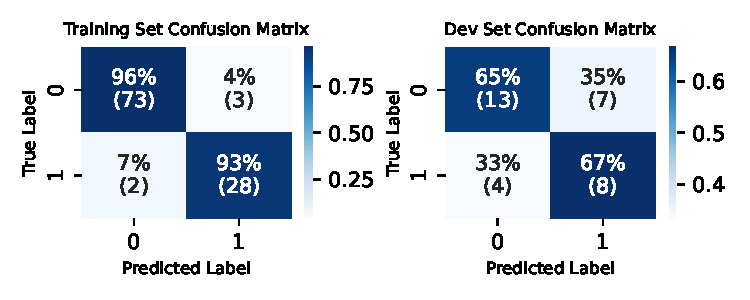
\includegraphics[width=0.55\textwidth]{vis_pdf/daic_all_confusion_matrices.pdf} % Adjust the scale to fit the page
\caption{Confusion Matrices for Development Set (DAIC-WOZ)}
\label{fig:confusion_matrices}
\end{figure}


EATD

%TRAIN



\begin{table}[H]
\centering
\label{table:classification_report_train_eatd}
\begin{tabular}{|c|c|c|c|c|}
\hline
\textbf{Class} & \textbf{Precision} & \textbf{Recall} & \textbf{F1-score} & \textbf{Support} \\ \hline
0              & 0.96               & 0.84            & 0.90              & 56               \\ \hline
1              & 0.74               & 0.93            & 0.82              & 27               \\ \hline
\multicolumn{5}{|c|}{\textbf{Accuracy}: 0.87 \textbf{of} 83}                        \\ \hline
\multicolumn{5}{|c|}{\textbf{Macro Avg}: Precision 0.85, Recall 0.88, F1-score 0.86} \\ \hline
\multicolumn{5}{|c|}{\textbf{Weighted Avg}: Precision 0.89, Recall 0.87, F1-score 0.87} \\ \hline
\end{tabular}
\caption{Classification Report on Training Set - EATD}
\end{table}

%TEST

\begin{table}[H]
\centering
\label{table:classification_report_dev}
\begin{tabular}{|c|c|c|c|c|}
\hline
\textbf{Class} & \textbf{Precision} & \textbf{Recall} & \textbf{F1-score} & \textbf{Support} \\ \hline
0              & 0.71               & 0.88            & 0.79              & 52               \\ \hline
1              & 0.54               & 0.27            & 0.36              & 26               \\ \hline
\multicolumn{5}{|c|}{\textbf{Accuracy}: 0.68 \textbf{of} 78}                        \\ \hline
\multicolumn{5}{|c|}{\textbf{Macro Avg}: Precision 0.62, Recall 0.58, F1-score 0.57} \\ \hline
\multicolumn{5}{|c|}{\textbf{Weighted Avg}: Precision 0.65, Recall 0.68, F1-score 0.64} \\ \hline
\end{tabular}
\caption{Classification Report on Development Set - EATD}
\end{table}

\begin{figure}[H]
\centering
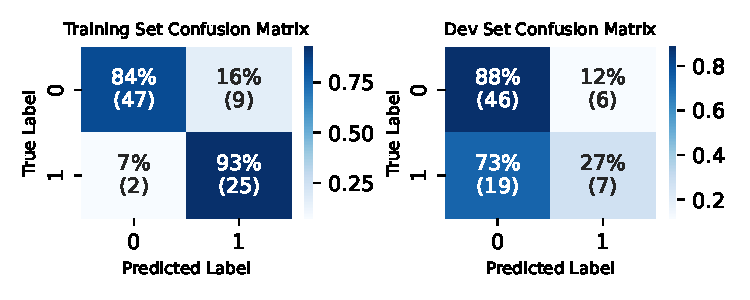
\includegraphics[width=0.55\textwidth]{vis_pdf/eatd_all_confusion_matrices.pdf} % Adjust the scale to fit the page
\caption{Confusion Matrices for Development Set (EATD)}
\label{fig:confusion_matrices}
\end{figure}

Worst to mention that when a DT was trained in both datasets the ANPVA choosed different features. 

\subsection{Model Performance - CNN}